\lhead{\emph{Servicios del sistema operativo}}
\chapter{Servicios del sistema operativo}

La complejidad que acarrea el uso de aplicaciones distribuidas hace necesario el uso de herramientas que permitan el desarrollo de forma cómoda del propio sistema, su uso posterior como herramienta de prueba de aplicaciones distribuidas y por último, facilitar el aprendizaje de algoritmos y herramientas distribuidas.

Muchas de las aplicaciones distribuidas utilizadas incluyen varias herramientas para facilitar su uso. Sin embargo estas soluciones suelen ser diseñadas para el propósito específico de dicha aplicación, y son difíciles de adaptar a otros contextos. Debido a esta carencia, se han creado varias herramientas propias que permiten aprovechar al máximo este sistema.

\section{MarcoPolo, el protocolo de descubrimiento de servicios}
\label{marcopolo}
Uno de los problemas típicos a la hora de crear un sistema distribuido es la localización de cada uno de los nodos que lo conforman. Soluciones como el uso de servidores de nombres (\textbf{DNS}) permiten crear estructuras jerárquicas donde cada nodo está identificado por un nombre previamente asignado y conocido. También existen protocolos inspirados en este como \textbf{mDNS} (\textit{Multicast Domain Name Service}) donde la necesidad de un servidor de nombres desaparece, y los nodos son capaces de realizar el descubrimiento mediante mensajes \textit{multicast}\cite{rfc6762}. Implementaciones de este protocolo, como \textit{Bonjour}, \textit{Avahi} o \textit{AppleTalk} (ya descontinuado) han sido evaluadas a la hora de buscar una solución a este problema.

Sin embargo, estas y otras soluciones similares no responden a una de las necesidades básicas del sistema a construir: la condición de que la información que conoce cada nodo sobre el resto en el arranque del sistema es nula. Si bien con \textbf{mDNS} desaparece la necesidad con un servidor de nombres y es posible realizar operaciones de descubrimiento de servicios, este y otros protocolos similares asumen que la información de un nodo presente de una red local es de interés para el resto de miembros de la misma, lo cual dificulta la independencia de un conjunto de equipos frente al resto en el mismo espacio de direcciones.

Una de las piezas clave del sistema consiste en la escalabilidad del mismo en tiempo de ejecución: no es necesario conocer qué nodos participan en el sistema hasta que no se requiera de los mismos. Además, se pretende optimizar al máximo cada uno de los nodos del sistema por separado, por lo que designar a uno de ellos como ``autoridad'' frente a la que el resto de nodos se registren y esta actúe posteriormente como nodo coordinador que actue como \textit{``resolver''} supone una dedicación de recursos innecesaria y que dificulta la escalabilidad del sistema. Además, la gestión del espacio de direcciones de la red en la que se integra el sistema no recae en este y además es compartido con una gran cantidad de equipos adicionales. Esto implica que las direcciones de cada nodo son asignadas por un servidor DHCP (\textit{Dynamic Host Configuration Protocol}) sobre el que no se tiene control, y cuyas asignaciones son dadas por intervalos de tiempo pequeños\footnote{Durante el desarrollo del sistema se observa que las direcciones son asignadas por periodos de tiempo pequeños y no suelen repetirse a menos que dicha dirección no haya sido asignada anteriormente, fenómeno que suele darse con bastante frecuencia.}. %TODOEsto implica que no es posible contar con un nodo coordinador sin un espacio de nombres anteriormente definido.
Por otro lado, la clave de este sistema no la constituye la disponibilidad de un nodo, sino las aplicaciones distribuidas que pueden utilizarse en el mismo (de ahora en adelante serán denominadas ``servicios''). Un nodo puede contar con un conjunto de servicios diferente al de sus vecinos, y por tanto colaborará en unas tareas y en otras no en virtud de dicha disponibilidad.%TODO Este requisito no es satisfecho por la mayoría de los sistemas anteriormente mencionados.

Motivada por esta serie de características surge la necesidad de crear un protocolo de descubrimiento de nodos basado principalmente en los servicios que dichos nodos pueden (y desean) ofrecer. Además, siendo uno de los objetivos funcionales del sistema el aprovechamiento del mismo como herramienta didáctica, surge la necesidad de que dos conjuntos de nodos puedan trabajar en la misma red de forma independiente. Como aproximación para satisfacer estas necesidades surge el procolo de descubrimiento de servicios \textbf{MarcoPolo}.

\subsection{MarcoPolo: Introducción}

MarcoPolo es un protocolo de descubrimiento de servicios cuya dinámica y nombre se inspiran en el juego homónimo\citationneeded, en el cual uno de los integrantes debe encontrar al resto privado de visión mediante ecolocalización (gritando la palabra clave ``Marco'', cuya respuesta por parte del resto de jugadores es ``Polo''). El protocolo se compone de dos roles claramente diferenciados (e independientes aún siendo ejecutados en el mismo nodo): \textbf{Marco}, encargado de enviar consultas a la red y \textbf{Polo}, que emite una respuesta a dichos comandos y gestiona la información de cada nodo. %TODO: http://en.wikipedia.org/wiki/Marco_Polo_%28game%29#cite_note-play-1.http://www.wisegeek.com/what-is-the-game-marco-polo.htm

Con el objetivo de posibilitar la coexistencia de varias ``mallas'' de nodos independientes (donde los servicios ofrecidos por un nodo sean conocidos y consecuentemente aprovechables únicamente por el resto) a la vez que las consultas son realizadas a todos los integrantes sin necesidad de conocer su identificador en la red (dirección a nivel de red o enlace, nombre \textit{DNS}) se utilizan mensajes uno-a-muchos, conocidos con el nombre \textit{multicast}, donde cada una de las ``mallas'' se comunicará con el resto de integrantes de la misma a través de un grupo preestablecido (o consensuado por dichos nodos).

\subsubsection{Objetivos}
\begin{itemize}%TODO
	\item Independencia
	El protocolo debe ser compatible con el mayor número de aplicaciones posible, adaptándose. Dicho objetivo se consigue delegando una gran parte de la funcionalidad a aplicaciones que se apoyan sobre el protocolo, en vez de implementar dicha funcionalidad en este. Dicho desacoplamiento permite, gracias a la mayor simplicidad del protocolo, poder ser compatible con un mayor número de casos de uso.
	\item \textit{Zeroconf}.
	El protocolo funciona en una red sin requerir ningún tipo de configuración por parte del usuario, y en una gran cantidad de casos, sin gran esfuerzo por parte del administrador. %TODO: http://en.wikipedia.org/wiki/Zero-configuration_networking
	\item Segmentación
	Varias instancias del protocolo pueden ejecutarse en una misma red de forma independiente, permitiendo la creación de varias ``mallas'' de equipos. Dicha segmentación no debe alterar en absoluto el esquema de la red preexistente.
	\item Conectable
	Las diferentes aplicaciones presentes en los diferentes nodos deben poder aprovechar la funcionalidad del protocolo mediante una serie de elementos conectores (interfaces).
	\item Seguro
	En aquellos casos en los que la información compartida por los nodos sea confidencial, el protocolo debe implementar las medidas oportunas para la protección de la misma.
	\item Independiente de plataforma e implementación
	Toda la comunicación entre elementos del protocolo se realizará a través de tecnologías que no dependan de una implementación concreta, tales como un lenguaje de programación o un sistema operativo dado. El único elemento que puede presentar tal dependencia es el conector final con otro código fuente, así como cualquier otro punto final (comandos, ficheros de configuración, etc).
	\item Independiente del espacio de direcciones, nombres de red y cualquier otro elemento
	El protocolo debe funcionar en cualquier espacio de direcciones dado, sin considerar en cualquier caso la dependencia con protocolos como \textbf{DHCP} o \textbf{DNS}.
	\item Simplicidad
	Los comandos del protocolo deben ser simples y, en caso de que sea posible, deben ser similares a otros ya conocidos por los usuarios del sistema, a fin de que estos ya estén familiarizados con los mismos.
	\item Descentralización
	El protocolo no debe en ningún momento generar un ``cuello de botella'', a menos que sea la opción más adecuada para la una tarea dada\footnote{Como se detalla más adelante, dichas situaciones se han desplazado a las aplicaciones que utilizan MarcoPolo}.
	\item Visibilidad
	\item Optimización de la red
	\item Sin conexión
	\item Extensible
	\item Extensible a diferente hardware
\end{itemize}

\subsection{Comandos}

El protocolo consiste en una serie de mensajes (a partir de ahora denominados \textit{comandos}) que contienen las consultas sobre la información de uno o varios servicios, nodos o información sobre la propia \textit{malla} que un nodo desee conocer, así como la respuesta a dichas consultas. Dichos mensajes son enviados como cadenas de texto que almacenan la información en estructuras de datos JSON (\textit{JavaScript Object Notation}) debido a la gran legibilidad de estas por humanos y la gran cantidad de herramientas disponibles para su creación y procesado.

Los comandos de MarcoPolo constituyen las primitivas del protocolo. Actualmente se cuenta con las siguientes primitivas y las correspondientes respuestas:
\begin{landscape}
\begin{table}[H]
\begin{tabular}{|p{1.5cm}|p{1.2cm}|p{5cm}|p{5cm}|p{5cm}|p{3.5cm}|}
\hline
Nombre & Emisor & Función & Información & Respuesta esperada & Protocolo y puerto\\ \hline
\textbf{Marco} & Marco & Descubrir todos los nodos presentes en la \textit{malla} & Únicamente se incluye el nombre del comando & Un comando \textit{Polo} por cada nodo disponible en la red, incluyendo como parámetros opcionales información sobre el nodo o \textit{ninguna} si no existe ningún nodo disponible. & UDP \textit{multicast} al puerto 1338.\\ \hline
\textbf{Polo} & Polo & Informar a un nodo de la existencia del emisor & Información sobre el nodo opcional (servicios disponibles, información sobre el nodo o la instancia de Polo\dots) & \textit{Ninguna} &  UDP \textit{unicast} al puerto efímero del mensaje de pregunta.\\ \hline
\textbf{Request-For} & Marco & Conocer todos los nodos que ofrecen un servicio identificado por su nombre único en el sistema & Identificador unívoco del servicio a descubrir & \textbf{OK} con información opcional sobre el nodo o el servicio & UDP \textit{multicast} al puerto 1338.\\ \hline
\textbf{OK} & Polo & Comando utilizado para emitir una respuesta a una petición, siendo la información de interés contenida en los parámetros de respuesta. & Respuesta a un comando con la información solicitada & \textit{Ninguna} & UDP \textit{unicast} al puerto efímero de la pregunta.\\ \hline
\textbf{Services} & Marco & Descubrir todos los servicios ofrecidos por un nodo & No se envía información adicional con el comando & \textbf{OK} con una lista de los identificadores del servicio o \textit{ninguna} si el nodo no está en la red. & UDP \textit{unicast} al puerto 1338.\\ \hline
\end{tabular}
\end{table}
\end{landscape}

\subsection{Esquemas de comunicación}

\subsubsection{Comando \textbf{Marco}}

\begin{figure}[H]
\centering
\includegraphics[width=\textwidth]{Diagrams/Sequence/marcocompleto}
\caption[Interacción al enviar el comando \textbf{Marco}]{Interacción al enviar el comando \textbf{Marco}. Los mensajes a grupos \textit{multicast} se indican con ``*''}
\label{fig:secuencia_marco}
\end{figure}

El comando Marco se envía al grupo \textit{multicast} definido en la configuración de la instancia local de \textbf{Marco}. Los nodos suscritos a dicho grupo (aquellos que pertenecen a la ``malla'') reciben el mensaje y emiten una respuesta \textbf{Polo}. Debido a la falta de una conexión entre los nodos (debido a que todos los mensajes son intercambiados utilizando el protocolo UDP) se fija un tiempo de espera de respuesta, durante el cual se reciben y acumulan todas las respuestas. Al final dicho tiempo de espera, se retornan los resultados y el resto de respuestas son ignoradas.

\begin{figure}[H]
	\centering
	\includegraphics[width=\textwidth]{Diagrams/Sequence/request_for}
	\caption[Interacción al enviar el comando \textbf{Request-For}]{Diagrama de interacción al enviar el comando \textbf{Request-For}. Los nodos comprueban si deben ofrecer el servicio identificado por la clave \textit{s}. En caso de que la búsqueda sea exitosa se retorna un mensaje indicando la disponibilidad de dicho nodo. En caso contrario no habrá respuesta alguna.
	Los mensajes enviados a grupos \textit{multicast} se indican con ``*''}
	\label{fig:secuencia_request_for}
\end{figure}

\begin{figure}[H]
	\centering
	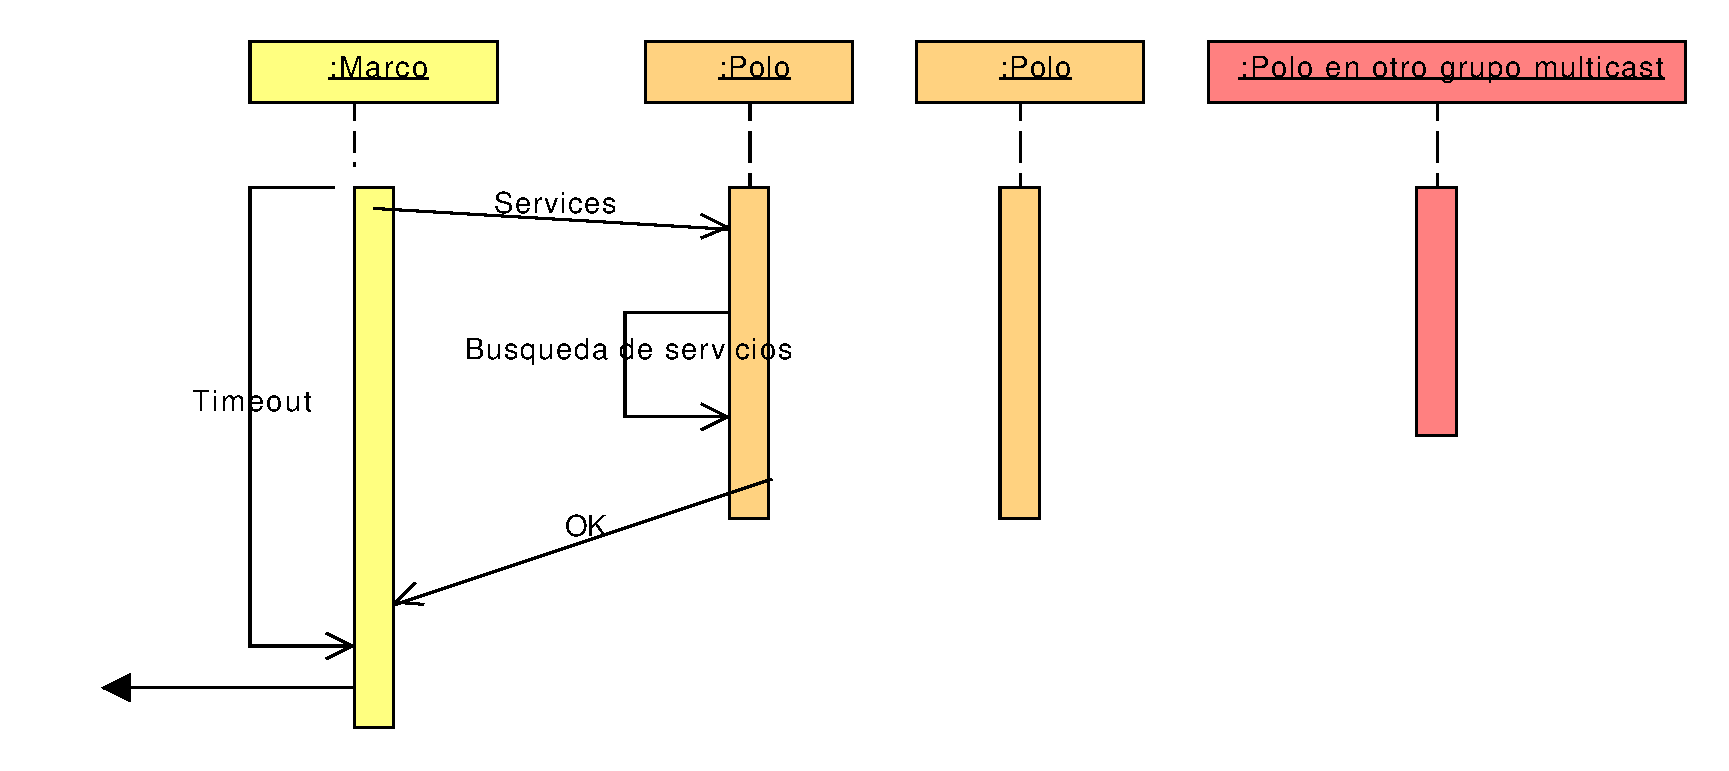
\includegraphics[width=\textwidth]{Diagrams/Sequence/services}
	\caption[Diagrama de interacción al enviar el comando \textbf{Services}]{Diagrama de interacción al enviar el comando \textbf{Services}. El nodo al que se le envía el comando consulta la información sobre los servicios que posee y posteriormente envía una respuesta a la instancia de Marco que ha realizado la consulta. Obsérvese toda la información es enviada en modo \textit{unicast}}
	\label{fig:secuencia_services}
\end{figure}

\subsection{Arquitectura en detalle}

La funcionalidad del protocolo se segmenta en dos roles claramente definidos e identificados: \textbf{Marco} y \textbf{Polo}. Dicha funcionalidad se implementa en dos ejecutables completamente independientes, que pueden por tanto coexistir o ser ejecutados sin presencia del otro elemento.

Dichos ejecutables son iniciados al arranque el equipo, aprovechando para ello las herramientas que el sistema operativo provee\footnote{Los ejecutables han sido configurados para ser compatibles con el inicializador \textbf{init} y el más reciente \textbf{systemd}.}, y se ejecutan en segundo plano de forma continua (es por ello pueden ser categorizados como procesos \textit{daemon}).

Toda la funcionalidad se ejecuta en un único proceso que se encarga de la creación de los diferentes canales de comunicación (utilizando la API de \textit{sockets} de Berkeley). Dichos canales de comunicación son gestionados por la utilidad \textbf{Twisted}\stepcounter{undefinedreferences}, que simplifica el trabajo con la API, en particular a la hora de crear \textit{sockets} asíncronos.

\subsubsection{Configuración}

Todos los aspectos modificables de cada rol, tales como el grupo \textit{multicast} al que suscribirse o el tiempo de espera predeterminado se definen en un archivo de configuración alojado en el directorio \texttt{/etc/marcopolo} (siguiendo la estructura definida en el \textit{Filesystem Hierarchy Standard} \cite{fhs}).

\begin{figure}[H]
	\centering
	\VerbatimInput{/home/martin/TFG/Documentación/memoria-tfg/memoria/Code/confdir.txt} %TODO
	\caption{Árbol de directorios dentro del directorio de configuración}
	\label{fig:arbol_marcopoloconf}
\end{figure}

Los archivos de configuración de cada uno de los \textit{daemons} sigue la típica estructura clave-valor presente en archivos de configuración de servicios del sistema. Por el contrario, la información de todos los servicios a ofrecer sigue la sintaxis de un fichero \textbf{JSON}\footnote{La razón de esta decisión de diseño es la facilidad de interpretación de dicho formato y la legibilidad que ofrecen.}. Todos estos ficheros son leídos al arrancar el ejecutable, y su modificación no tendrá efectos hasta la próxima vez que se inicie el servicio (salvo excepciones que veremos a continuación).

\javascriptcode{statusmonitor}{Un archivo que describe el servicio status monitor}{1}{4}

\subsubsection{Archivos auxiliares}

\paragraph{Log}
Toda la información sobre la ejecución de los \textit{daemons} se refleja en los archivos de \textit{log} presentes en el directorio \texttt{/var/log/marcopolo}. El nivel de log se configura en el parámetro \texttt{LOGLEVEL} de cada uno de los \textit{daemons} y puede tomar uno de los siguientes valores:

\begin{itemize}
\item \textbf{Error} Errores internos durante la ejecución.
\item \textbf{Warn} Advertencias sobre posibles situaciones atípicas.
\item \textbf{Info} Información de interés sobre el funcionamiento del sistema.
\item \textbf{Debug} Información de depuración.
\end{itemize}

%\logcode{/home/martin/TFG/Documentación/memoria-tfg/memoria/Code/marcod}{Caption}{1}{3} %TODO

\paragraph{Registro de ejecución}

En ocasiones es necesario conocer el identificador del proceso \textbf{PID} del \textit{daemon}. Para ello se almacena en el directorio \texttt{/var/run/marcopolo/(marco.pid|polo.pid)} dicho identificador, que puede ser aprovechado por el gestor de arranque del proceso.

\subsection{Integración de los \textit{daemons} en el sistema operativo}

Los \textit{daemons} se integran en el arranque del sistema a través de los ficheros de configuración de \texttt{init}\citationneeded{} o \texttt{systemd} dependiendo del gestor disponible en el sistema operativo sobre el que se ejecuten los procesos.

Por defecto los \textit{daemons} se ejecutan durante todo el ciclo de vida del computador, pero pueden ser reiniciados o detenidos arbitrariamente por voluntad del administrador:

\begin{lstlisting}
systemctl start (marco|polo)
systemctl stop (marco|polo)
systemctl restart (marco|polo)
systemctl reload polo #Orden exclusiva de Polo
\end{lstlisting}

El comando \texttt{reload} permite actualizar la lista de servicios que \textbf{Polo} ofrece sin tener que detener todo el proceso para ello. Dicho comportamiento se consigue de forma similar al comando \texttt{reload} de Apache, enviando la señal \texttt{SIGUSR1} al proceso. 

\subsection{Conexiones con MarcoPolo (\textit{Bindings})}

La funcionalidad de \textbf{MarcoPolo} no se limita al descubrimiento de los servicios del sistema, por lo que es necesario proveer a los usuarios del clúster de herramientas que permitan integrar sus aplicaciones distribuidas con estos servicios. Dichas herramientas, conocidas generalmente como \textit{bindings}, permiten exponer públicamente la funcionalidad de \textbf{MarcoPolo} para que pueda ser aprovechada por otros usuarios.

Se han creado \textit{bindings} para los lenguajes de programación \textbf{Python} y \textbf{Java} y se plantea crear uno para el lenguaje \textbf{C}. Todos ellos son consistentes entre sí, y utilizan la misma sintaxis para realizar el mismo tipo de operación a la vez que aprovechan las características propias de cada lenguaje. Dicha filosofía está inspirada en el funcionamiento de las primitivas de la API de resolución de nombres en red (\texttt{netdb.h})\cite{netdb}, por lo que los \texttt{bindings} se comunican con la instancia local de Marco o Polo a través de \textit{sockets} vinculados a la dirección IP local (127.0.1.1).

Todos los \textit{bindings} deben implementar el mismo conjunto de primitivas, a saber:

\paragraph{Primitivas en el \textit{binding} de Marco}
\begin{itemize}
\item \texttt{request\_for(service, timeout=None)}
Retorna una lista de nodos que ofrecen el servicio indicado en \texttt{service}. Esta función bloquea la ejecución del proceso hasta que el tiempo de espera de nuevas respuestas se cumple (si bien esto no constituye un problema para la mayoría de aplicaciones, es importante que sea conocido por el programador). Si se especifica un \texttt{timeout}, este se utiliza en lugar del determinado por defecto en los parámetros de configuración de \textbf{MarcoPolo}. Se lanza una excepción o un código de error en caso de que la comunicación con la instancia de \textbf{Marco} sea infructuosa (generalmente este tipo de problemas se originan debido a un fallo en el arranque del servicio). Toda la información es transferida en cadenas JSON codificadas en UTF-8.


\item \texttt{getOneNode(criteria=None, timeout=None)}

Retorna un nodo elegido aleatoriamente entre las respuestas (en concreto, el nodo cuya respuesta llegue primero). Si se especifica un criterio en la variable \texttt{criteria} se elegirá el nodo que mejor satisfaga dicho criterio. %TODO in sphinx and MarcoPolo

\item \texttt{getAllNodes(timeout=None)}
Retorna todos los nodos disponibles en la \textit{malla} sin considerar los servicios ofertados. Se lanza una excepción o un código de error en caso de que la comunicación con la instancia de \textbf{Marco} sea infructuosa.

\item \texttt{getNodeInfo(ip)} %TODO Timeout
Obtiene la información de un nodo identificado por su \texttt{ip} si este está disponible en la red.

\end{itemize}

\paragraph{Primitivas en el \textit{binding} de Polo}

\begin{itemize}
\item \texttt{register\_service(service, params=None)}

Añade un nuevo servicio al conjunto de servicios ofertados. El servicio únicamente será ofertado durante el ciclo de vida de la instancia local de Polo. Si esta es detenida o reiniciada se procederá a la eliminación del registro. Para registrar un servicio de forma permanente es necesario definirlo en el directorio \texttt{/etc/marcopolo} %TODO add section reference.

\item \texttt{remove\_service(service)}
Elimina un servicio de la lista de ofertados. Para poder realizar este proceso es necesario ser el ``propietario'' del servicio. Esto es, el único proceso que puede eliminar un servicio es aquel que lo creó o en su defecto la instancia de \textbf{Polo}. En caso de que esta restricción sea quebrantada, una excepción o código de error será retornado.

\item \texttt{have\_service(service)}
Indica si el servicio está ofertado o no.

\end{itemize}

Como se puede observar, la mayoría de primitivas tienen como objetivo el descubrimiento y publicación de servicios. Sin embargo, varias de ellas permiten realizar consultas sobre la información del propio nodo y se plantea la creación de más primitivas que sigan dicha filosofía.

\section{Aplicaciones construidas sobre MarcoPolo}
 
\subsection{Utilidades}

A fin de simplificar al máximo el funcionamiento de los \textit{daemons} varias utilidades que podrían tener cabida dentro del propio protocolo han sido creadas como utilidades independientes que aprovechan la funcionalidad de \textbf{MarcoPolo} para realizar su cometido, pero cuya interdependencia se limita a dichos canales de comunicación.

\subsubsection{\texttt{marcodiscover}}
\label{marcodiscover}
Esta utilidad consiste en un comando que permite ejecutar consultas al sistema a través de un intérprete de órdenes. El comando posibilita realizar la mayoría de consultas de interés y cuenta con varias opciones para dar diferentes formatos a la salida por pantalla, algo que, como veremos posteriormente, es de gran utilidad para la ejecución de un conjunto particular de programas.

Las opciones del comando son las siguientes:

\begin{figure}[H]
\centering
\begin{lstlisting}
usage: marcodiscover.py [-h] [-d [ADDRESS]] [-s [SERVICE]] [-S [SERVICES]]
                        [-n [NODE]] [--sh [SHELL]]

Discovery of MarcoPolo nodes in the subnet

optional arguments:
  -h, --help            show this help message and exit
  -d [ADDRESS], --discover [ADDRESS]
                        Multicast group where to discover
  -s [SERVICE], --service [SERVICE]
                        Name of the service to look for
  -S [SERVICES], --services [SERVICES]
                        Discover all services in a node
  -n [NODE], --node [NODE]
                        Perform the discovery on only one node, identified by
                        its ip/dns name
  --sh [SHELL], --shell [SHELL]
                        Print output so it can be used as an interable list in
                        a shell

\end{lstlisting}
\caption{Opciones de configuración de \texttt{marcodiscover}}
\label{fig:marcodiscover_help}
\end{figure}

\subsubsection{Marcoinstallkey}
\label{marcoinstallkey}

\subsection{Aplicaciones construidas sobre MarcoPolo}

A fin de aprovechar la funcionalidad de \textbf{MarcoPolo} dentro del sistema, se crean las siguientes utilidades

\subsubsection{Status Monitor}

El monitor de estado consiste en una aplicación con interfaz web que permite observar las estadísticas de uso del \textit{hardware} y de diversos procesos. Utiliza para la detección de los diferentes nodos el \textit{binding} de \textbf{Marco} en Python que realiza una consulta para descubrir que nodos están dispuestos a ofrecer el servicio \texttt{statusmonitor}. La respuesta de dicho comando es enviada al cliente, que establece conexiones directas a cada uno de los nodos a través de \textit{Websockets}\citationneeded. Esto es posible debido a que según la especificación del estándard de websockets, la \textit{Same-Origin Policy}\cite{rfc6455} no es utilizada de la misma forma que en peticiones HTTP,\cite{rfc6454}.

\begin{figure}[H]
\centering
\includegraphics[width=\textwidth]{Diagrams/Sequence/statusmonitor}
\caption[Interacción completa del usuario con \textbf{Statusmonitor}]{Interacción completa del usuario con \textbf{statusmonitor}. Los mensajes a grupos \textit{multicast} se indican con ``*''}. El usuario se conecta a la página web, que en respuesta envía un código \textit{JavaScript} (además del código HTML y CSS) que solicita la lista de nodos disponibles. Una vez recibida la petición de los nodos disponibles, el servidor solicita dicha información a través de su instancia local de \textbf{Marco} (utilizando para ello un \textit{binding}. Cuando la instancia de \textbf{Marco} termina de recoger las respuestas, retorna la información al servidor, que a su vez retorna dicha información al cliente. Al recibir dicha información, el nodo crea una conexión \textit{Websocket} con el servicio statusmonitor que se encarga de enviar por dicha conexión la información local a intervalos de tiempo definidos.)
\label{fig:secuencia_statusmonitor}
\end{figure}

\begin{figure}[H]
	\centering
	\includegraphics[width=\textwidth]{Chapter7/Figures/statusmonitor}
	\caption[Vista de la interfaz web de \textbf{Statusmonitor} una vez obtenidos los nodos]{Vista de la interfaz web una vez obtenidos los nodos y establecida la conexión a los mismos. Se observa el porcentaje de memoria y principal y de intercambio utilizadas, la temperatura del procesador, los procesos con más consumo de CPU} %TODO: y el porcentaje de CPU utilizado en cada núcleo.
	\label{fig:vista_statusmonitor}
\end{figure}

Para conocer la información sobre el sistema el proceso servidor utiliza varios comandos y ficheros auxiliares, destacando:

\begin{itemize}
\item \texttt{top} Para conocer la información sobre los procesos más activos
\item El directorio \texttt{/proc} para conocer estadísticas del sistema como la memoria total, libre y en caché
\item El directorio \texttt{/sys} para conocer características del hardware como la temperatura
\item Comandos como \texttt{uptime} o \texttt{hostname} para conocer diversos parámetros del sistema.
\item Herramientas como \texttt{awk}, \texttt{grep} o \texttt{cut} para obtener las cadenas de interés dentro del comando de respuesta.
\end{itemize}

Dichos comandos son ejecutados periódicamente mediante el gestor de eventos \texttt{ioloop} de \textbf{Tornado}.

La implementación del servicio está realizada íntegramente en Tornado\footnote{Más información sobre el proyecto puede encontrarse en \href{http://www.tornadoweb.org/en/stable/}{tornadoweb.org/en/stable}}, un servidor web ligero asíncrono implementado íntegramente en Python y mantenido por Facebook.

\subsubsection{Deployer}

El \textbf{Deployer} es una herramienta concebida a partir de la necesidad observada entre los estudiantes de las asignaturas Sistemas Distribuidos y Arquitectura de Computadores (como se refleja en las diferentes evaluaciones\citationneeded %TODO
realizadas), de replicar de una forma sencilla un ejecutable entre los diferentes nodos que conformarán el sistema distribuido.

Actualmente la infraestructura cuenta con un servidor NFS que posibilita la disponibilidad de la información en varios nodos de forma sencilla, mediante la copia a uno de los directorios alojados en el servidor. Sin embargo, este enfoque presenta varios inconvenientes: en el aspecto técnico supone una gran cantidad de ancho de banda consumido de forma continua (debido a que todos los estudiantes utilizan la misma infraestructura y realizan un gran número de operaciones de lectura y escritura a estos directorios, ralentizando el funcionamiento general del sistema enormemente) y en el aspecto didáctico, fomenta un mal hábito, pues los estudiantes no conocen otra forma de realizar despliegues más allá de la copia utilizando una interfaz gráfica y accediendo físicamente al nodo (si bien esta situación se mitiga en la asignatura Sistemas Distribuidos, donde deben automatizar los despliegues). Además, es necesario disponer de acceso físico a cada uno de los nodos, o en su defecto, conocer sus direcciones de red para realizar un acceso remoto.

Con el objetivo de proporcionar una alternativa adecuada a las necesidades y problemas descritos, surge esta herramienta, que aprovecha la funcionalidad de \textbf{MarcoPolo} para realizar su cometido.

La herramienta permite realizar las siguientes tareas de forma sencilla:

\begin{itemize}
\item Conocer todos los nodos disponibles sobre los que se podrá realizar el despliegue y seleccionar sobre cuáles de ellos trabajar.
%\item Conocer la situación de cada nodo en tiempo real, aprovechando la herramienta \textbf{statusmonitor}, cuya funcionalidad se integra en este sistema.
\item Permitir la copia a dichos nodos.
\item Posibilitar la ejecución de comandos de forma remota una vez que el despliegue ha sido realizado.
\item Facilitar la integración con contenedores de servicios, tales como \textbf{Apache Tomcat}.
\end{itemize}

La aplicación es accesible a través de un panel web %TODO: o del comando marcodeploy
. La interfaz web permite además conocer el estado de cada nodo en tiempo real, funcionalidad que a través de la línea de órdenes está disponible a través de los comandos %TODO: marcostatus

\begin{figure}[H]
\centering
\includegraphics[width=\textwidth]{Chapter7/Figures/deployer}
\caption[Interfaz web del deployer]{Interfaz web del deployer. A la izquierda figuran los controles y a la derecha la lista de nodos sobre los que se puede realizar el despliegue}
\label{fig:vista_deployer}
\end{figure}

Al igual que en el caso de la aplicación \textbf{statusmonitor} el \textbf{deployer} está creado utilizando el servidor web \textbf{Tornado} y todo el contenido enviado al usuario se reduce a archivos HTML, CSS y JavaScript. La comunicación entre el cliente y el servidor se realiza a través de peticiones \textit{AJAX} y \textit{Websockets}. Todo el control de la interfaz se delega a hojas de estilo CSS y JavaScript utilizando la biblioteca jQuery\footnote{\href{https://jquery.com/}{jquery.com/}}.

\paragraph{Autenticación}

La autenticación de los usuarios se realiza mediante el módulo \textbf{PAM} presente en cada nodo\citationneeded{}, utilizando \textbf{python-pam} para el acceso al mismo desde \textbf{Python}\cite{python-am}.

%TODO: \begin{figure}[H]
% \centering
% %\includegraphics[width=\textwidth]{Chapter7/Sequence}
% %\caption{Diagrama de secuencia de la interacción}
% %\label{fig:sequence_deployer}
% \end{figure}

\subsection{Herramientas de gestión}

\subsubsection{pam\_mkhomedir}
\label{pam_mkpolohomedir}

\textbf{PAM} permite ampliar la funcionalidad que ofrece por defecto mediante la inclusión de \textit{módulos}, pequeñas bibliotecas compartidas de código con las acciones a realizar.

Uno de los módulos incluidos en la instalación por defecto de \textbf{PAM} es \textbf{mkhomedir}, encargado de la creación de un directorio propio para el usuario en caso de que aún no se haya realizado dicha acción. El proceso consiste en una copia del directorio \textbf{skeleton} (generalmente situado en \texttt{/etc/skel}) y la correcta fijación de permisos en el mismo.

Sin embargo, el directorio únicamente es creado en el nodo al que se accede. La filosofía del proyecto se basa en la creación de un sistema que se componga de varias unidades, pero se comporten como una única entidad, por lo que obligar al usuario a acceder a todos los nodos para poder trabajar en el sistema completo rome dicha transparencia. Es por ello necesario contar con un sistema que extienda la funcionalidad de \textbf{mkhomedir} para incluir el resto de nodos en la creación del directorio.

Con este objetivo nace \textbf{pam\_mkpolopohomedir}, un módulo basado en \textbf{mkhomedir} que hace uso de \textbf{MarcoPolo} para detectar los nodos presentes en la red que ofrezcan el servicio \texttt{polousers} y solicitar a los mismos la creación del directorio de inicio.

El módulo se implementa en C/C++ debido a que es el lenguaje con el que los módulos de PAM se construyen por defecto y utiliza por tanto el \textit{binding} de MarcoPolo para este lenguaje. Existen sin embargo herramientas para desarrollar el mismo en Python\footnote{\citationneeded{python-pam}}.

Un módulo en PAM debe implementar una serie de funciones que constituirán los puntos de entrada al módulo\citationneeded{pam manpages}:

\begin{itemize}
\item \texttt{PAM\_EXTERN int pam\_sm\_open\_session(pam\_handle\_t \* pamh, int flags, int argc ,const char **argv)}\\

Es la función que \textbf{PAM} invoca al incluir el módulo. Incluye en el mismo una estructura \texttt{pam\_handle\_t} con toda la información relevante sobre el usuario que ha iniciado sesión y los parámetros indicados en los ficheros de configuración de \texttt{PAM} (en el caso de este módulo, los permisos del directorio de inicio y la localización del directorio \textit{skeleton}). 

%comoPpunto de entrada al móduloal inicialmente

\item \texttt{PAM\_EXTERN int pam\_sm\_close\_session(pam\_handle\_t * pamh, int flags, int argc, const char **argv)}

Es la función que \textbf{PAM} utiliza para indicar al módulo que la sesión ha terminado. En el caso del módulo a crear no se debe realizar ninguna acción en este evento, sin embargo es necesario implementarla debido a que PAM la requiere.

\item \texttt{struct pam\_module \_pam\_mkhomedir\_modstruct}

Define las características del módulo y los puntos de entrada que define.
\end{itemize}

El módulo realiza la siguiente secuencia de pasos:

\begin{enumerate}
\item Determina la información de interés a partir de los datos provistos por \textbf{PAM} y las acciones a llevar a cabo. En caso de que el directorio ya exista, se omite la creación del mismo y únicamente se solicita la creación en el resto de nodos\footnote{Este paso siempre es necesario para facilitar la expansibilidad del sistema: añadir un nuevo nodo tras la creación del directorio en el resto haría que este no fuera accesible de no ser por la repetición de este paso}.
\item Realiza si es necesaria la creación del directorio en el nodo actual.
\item Detecta con \textbf{MarcoPolo} el resto de nodos dispuestos a colaborar en el sistema (aquellos que oferten el servicio \textbf{polousers}).
\item Solicita a cada uno de ellos la creación del directorio.
\item Una vez que todos los nodos han realizado la acción solicitada, se da acceso al sistema.
\end{enumerate}

Todas las operaciones realizan escrituras en ficheros de \textbf{log} para su posterior análisis.

\paragraph{Seguridad}

Al tratarse de acciones llevadas a cabo por usuarios con privilegios elevados y que involucran la gestión de información personal, todas las comunicaciones se realizan utilizando conexiones cifradas mediante \textit{sockets} \textbf{TLS} (\textit{Transport Layer Security}) con certificados en ambos lados de la conexión, que son verificados por el contrario.

\paragraph{Extensibilidad}

El módulo ha sido diseñado con el objetivo de posibilitar la adición de nueva funcionalidad al mismo. Únicamente es necesario definir las acciones a llevar a cabo en el servicio \textbf{polousers} y solicitar su realización mediante la sintaxis de comandos de \textbf{MarcoPolo}.

\subsubsection{MarcoBootstrap}

Uno de los mayores problemas a la hora de gestionar un sistema con un número de componentes elevado es la instalación de todos los componentes y la actualización de los mismos. \textbf{MarcoBootstrap} es una herramienta que posibilita la instalación del sistema operativo de forma autónoma y que únicamente requiere la copia en la tarjeta SD del sistema de un pequeño conjunto de utilidades, cuyo tamaño es 33 \textit{megabytes}.

%\ref{marcobootstrap}

\subsubsection{Marcologger}
\subsection{Herramientas didácticas}

\subsubsection{The LED API}

\subsubsection{MusicPI}


\subsection{Pruebas de concepto}

%\includegraphics{Chapter7/ScreenShot.png}http://www.bootc.net/archives/2012/05/26/how-to-build-a-cross-compiler-for-your-raspberry-pi/